\section{Verifica di ipotesi, t-statistica e p-value}

\subsection{Verifica d'ipotesi}

Lo standard error può essere utilizzata per effettuare la \textit{verifica d'ipotesi} su i coefficienti. La verifica di ipotesi più comune riguarda la verifica dell'\textit{ipotesi nulla}

\begin{equation}
H_0: \text{non c'è relazione tra X e Y}
\end{equation}

contro l'\textit{ipotesi alternativa}

\begin{equation}
H_1: \text{c'è qualche relazione tra X e Y}.
\end{equation}

Dal punto di vista matematico, questo corrisponde a testare

\begin{equation}
H_0: {\beta}_1 = 0
\end{equation}

contro

\begin{equation}
H_1: {\beta}_1 \neq 0
\end{equation}

visto che se ${\beta}_1 = 0$ allora il modello si riduce a $Y = {\beta}_0 + \epsilon$, e $X$ non è associata con Y. Per verificare l'ipotesi nulla dobbiamo determinare se $\overline{{\beta}_1}$, la nostra stima di ${\beta}_1$, è sufficientemente distante da $0$, in modo che possiamo essere sicuri che ${\beta}_1$ non sia zero. Questo dipende dall'accuratezza di ${\beta}_1$, che dipende da $SE({\beta}_1)$. Se è piccolo allora anche valori relativamente piccoli di ${\hat{\beta}}_1$ possono fornire una forte evidenza che ${\beta}_1 \neq 0$ e quindi che c'è una relazione tra $X$ e $Y$. Al contrario, se $SE({\beta}_1)$ è grande allora ${\hat{\beta}}_1$ deve essere grande in valore assoluto per poter rigettare la nostra ipotesi nulla.

\subsection{t-statistica}

In pratica, calcoliamo la \textit{t-statistica}, data da

\begin{equation}
t = \frac{{\hat{\beta}}_1 - 0}{SE({\hat{\beta}}_1)}
\end{equation}

che misura il numero di deviazioni standard di ${\hat{\beta}}_1$ che differiscono da $0$ e che sotto l'ipotesi nulla ha distribuzione $t_{n-2}$. Se non c'è alcuna relazione tra X e Y, allora ci aspettiamo che l'equazione precedente abbia una \textit{t-distribuzione} con $n - 2$ gradi di libertà. La distribuzione ha una forma a campana e per valori di $n$ più grandi di 30 è molto simile alla distribuzione normale.

Si rifiuta l'ipotesi nulla al livello di significatività $\alpha$ prefissato se il valore osservato di t

\begin{equation}
|t^{oss}| > t_{{\alpha}/2;n-2}.
\end{equation}

I test per valutare se un parametro si possa considerare pari a 0 si chiamano \textit{test di significatività}.

Ci sono della alternative unilaterali:

\begin{itemize}
\item $H_{0}: {\beta}_1 = 0 \text{ o } H_{0}: {\beta}_1 <= 0 \text{ vs } H_{1}:{\beta}_1 > 0$. La statistica test rimane la stessa. Si rifiuta l'ipotesi nulla al livello di significatività $\alpha$ se
\begin{equation}
t^{oss} > t_{1-\alpha;n-2}
\end{equation}
\item $H_{0}: {\beta}_1 = 0 \text{ o } H_{0}: {\beta}_1 >= 0 \text{ vs } H_{1}:{\beta}_1 < 0$. La statistica test rimane la stessa. Si rifiuta l'ipotesi nulla al livello di significatività $\alpha$ se
\begin{equation}
t^{oss} < t_{\alpha;n-2}
\end{equation}
\end{itemize}

La verifica d'ipotesi precedente si applica anche nel caso in cui si testino valori di ${\beta}_1$ e (${\beta}_0$) diversi da 0. In generale per $H_0: {\beta}_1 = {{\beta}_1}^{H_0}$ contro ${\beta}_1 \neq {{\beta}_1}^{H_0}$ si usa la statistica test

\begin{equation}
t = \frac{{\hat{\beta}}_1 - {{\beta}_1}^{H_0}}{SE({\hat{\beta}}_1)}
\end{equation}

che sotto l'ipotesi nulla ha distribuzione $t_{n-2}$.

\subsection{p-value}

È semplice calcolare la probabilità di osservare un valore maggiore o uguale di $|t|$, assumendo ${\beta}_0$. Chiamiamo questa probabilità \textit{p-value} o ${\alpha}^oss$. Interpretiamo il p-value come segue: un valore piccolo indica che è improbabile osservare un'associazione tra $X$ e $Y$ dovuta al caso caso, in assenza di una reale associazione tra  $X$ e $Y$. Rifiutiamo l'ipotesi nulla (dichiariamo che esiste una relazione tra $X$ e $Y$) se il p-value è sufficientemente piccolo.

Il p-value può essere interpretato come la probabilità di osservare per la statistica test valori almeno tanto estremi
quanto quello osservato sotto $H_0$, nella direzione di $H_1$. In alternativa, può essere considerato il più piccolo \textit{livello di significatività} che conduce al rifiuto di $H_0$.



\begin{itemize}
\item $H_{0}: {\beta}_1 = {{\beta}_1}^{H_0}$ contro $H_{0}: {\beta}_1 \neq {{\beta}_1}^{H_0}$. Dato $t^{oss}$ il valore osservato di $t$, si calcola ${\alpha}^{oss}$ come \begin{equation}
{\alpha}^{oss} = 2\min{P(t_{n-2} > t^{oss}),P(t_{n-2} < t^{oss})}
\end{equation}
\item $H_{0}: {\beta}_1 < {{\beta}_1}^{H_0}$ contro $H_{0}: {\beta}_1 >= {{\beta}_1}^{H_0}$
\begin{equation}
{\alpha}^{oss} = P(t_{n-2} > t^{oss})
\end{equation}
\item $H_{0}: {\beta}_1 >= {{\beta}_1}^{H_0}$ contro $H_{0}: {\beta}_1 < {{\beta}_1}^{H_0}$
\begin{equation}
{\alpha}^{oss} = P(t_{n-2} < t^{oss})
\end{equation}
\end{itemize}

In modo analogo si procede per ${\beta}_0$

\begin{figure}[H]
\centering
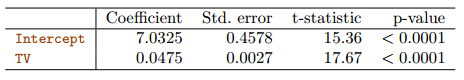
\includegraphics[scale=0.5]{t_stat_p_value}
\caption{t-statistica e p-value per il problema dell'Advertising}
\end{figure}